\documentclass[border=4pt]{standalone}
% Preámbulo común de las figuras. Cada figura es un documento standalone
% que se compila a SVG con scripts/build_figures.sh
\usepackage[utf8]{inputenc}
\usepackage{amsmath}
\usepackage{tikz}
\usepackage[american, siunitx]{circuitikz}
\usetikzlibrary{arrows.meta,calc,decorations.pathmorphing,patterns}
\tikzset{
  >={Stealth[length=2.2mm]},
  eje/.style={->, thin},
  hilo/.style={thick},
}
% Paleta común: tonos medios legibles sobre fondo claro
\definecolor{azul}{RGB}{31,94,168}
\definecolor{rojo}{RGB}{192,57,43}
\definecolor{verde}{RGB}{39,128,73}
\definecolor{naranja}{RGB}{211,120,30}
\definecolor{morado}{RGB}{125,60,152}

\begin{document}
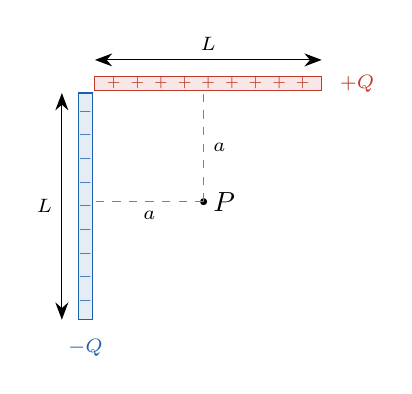
\begin{tikzpicture}[scale=3.0]
  \filldraw[draw=rojo, fill=rojo!12] (0.04,-0.03) rectangle (1.0,0.03);
  \foreach \s in {0.12,0.22,...,0.95} \node[text=rojo, font=\tiny, inner sep=0pt] at (\s,0) {$+$};
  \filldraw[draw=azul, fill=azul!12] (-0.03,-1.0) rectangle (0.03,-0.04);
  \foreach \s in {0.12,0.22,...,0.95} \node[text=azul, font=\tiny, inner sep=0pt] at (0,-\s) {$-$};
  \fill (0.5,-0.5) circle (0.015) node[right]{$P$};
  \draw[dashed, gray] (0.5,-0.5) -- (0.5,-0.04) (0.5,-0.5) -- (0.04,-0.5);
  \node[font=\scriptsize, right] at (0.5,-0.27) {$a$};
  \node[font=\scriptsize, below] at (0.27,-0.5) {$a$};
  \draw[<->, thin] (0.04,0.1) -- node[above, font=\scriptsize]{$L$} (1.0,0.1);
  \draw[<->, thin] (-0.1,-0.04) -- node[left, font=\scriptsize]{$L$} (-0.1,-1.0);
  \node[text=rojo, font=\scriptsize] at (1.15,0) {$+Q$};
  \node[text=azul, font=\scriptsize] at (0,-1.12) {$-Q$};
\end{tikzpicture}
\end{document}
